%TODO valutare se fare relativi UC per inserimento mail ed inserimento password.
%TODO da rifare gli indici (abbiamo saltato l'indice 5)

\subsection{UC- Login tramite applicazione mobile}
\begin{itemize}
	\item \textbf{Attore primario:} utente non autenticato;

	\item \textbf{Descrizione:} l'utente vuole autenticarsi presso il sistema da applicazione mobile tramite l'inserimento del proprio indirizzo e-mail di registrazione e la propria password;

	\item \textbf{Precondizioni:} l'utente è registrato ma non ha ancora eseguito l'accesso presso il sistema, l'utente ha avviato l'applicazione mobile;

	\item \textbf{Postcondizioni:} l'utente è autenticato presso il sistema;
%TODO creazione sottocasi mail e password per l'inserimento ed errore mail non presente.
	\item\textbf{Scenario principale:}
	      \begin{enumerate}
		      \item l'utente seleziona la funzionalità "Accedi";
		      \item l'utente inserisce il proprio indirizzo e-mail con il quale si è registrato presso il sistema;
		      \item l'utente inserisce la propria password;
		      \item l'utente invia i dati al sistema;
		      \item il sistema elabora la richiesta e aggiorna la schermata del dispositivo con la dashboard personale qualora il login venga eseguito con successo. In caso contrario il sistema restituisce un messaggio d'errore 			      esplicativo e non completa il login dell'utente(UC- Errore: inserimento di una coppia di credenziali non riconosciuta dal sistema).
	      \end{enumerate}
	\item \textbf{Estensioni:}
	      \begin{enumerate}
		      \item UC- Errore: inserimento di una coppia di credenziali non riconosciuta dal sistema.
	      \end{enumerate}
\end{itemize}

\subsubsection{UC-.1 Inserimento delle credenziali per effettuare il login tramite applicazione mobile}
\begin{itemize}
	\item \textbf{Attore primario:} utente non autenticato;

	\item \textbf{Descrizione:} l'utente vuole inserire le proprie credenziali (mail e password) per autenticarsi nell'applicazione mobile;

	\item \textbf{Precondizioni:} l'utente è registrato presso il sistema ed ha avviato l'applicazione mobile;

	\item \textbf{Postcondizioni:} l'utente ha inserito correttamente email e password;

	\item \textbf{Scenario principale:}
	      \begin{enumerate}
		      \item il sistema elabora la richiesta ricevuta;
		      \item il sistema restituisce un messaggio d'errore esplicativo che viene visualizzato sullo schermo dell'utente e non completa l'accesso.
	      \end{enumerate}
	\item \textbf{Estensioni:}
		\begin{enumerate}
		      \item UC- Errore: inserimento di una coppia di credenziali non riconosciuta dal sistema da applicazione mobile.
	      \end{enumerate}
\end{itemize}

\subsubsection{UC- Errore: inserimento di una coppia di credenziali non riconosciuta dal sistema da applicazione mobile}
\begin{itemize}
	\item \textbf{Attore primario:} utente non autenticato;

	\item \textbf{Descrizione:} l'utente ha inserito una coppia di credenziali in cui l'indirizzo mail o password sono errate o non censite all'interno del sistema. Il sistema non permetterà quindi il login;
	
	\item \textbf{Precondizioni:} l'utente ha inserito una coppia di credenziali (indirizzo mail e password) non censita all'interno del sistema;

	\item \textbf{Postcondizioni:} il sistema non accetta l'indirizzo email o password fornito dall'utente restituendo un errore esplicativo a video;

	\item \textbf{Scenario principale:}
	      \begin{enumerate}
		      \item l'utente seleziona i campi dati dove inserire la propria mail e password;
		      \item l'utente inserisce una mail o password non presenti o non associate all'interno del sistema;
		      \item il sistema visualizza un messaggio di errore esplicativo e non permette il login dell'utente.
		\end{enumerate}
\end{itemize}


%TODO da modificare con la One Time Password. Aggiungere UC per invio dati da parte dell'admin all'utente. da aggiungere UC-1.4 per inserimento password temporanea da parte dell'amministratore.
%TODO mettere prima login utente, poi rifare tutti gli indici.
\subsection{UC- Recupero password}
\begin{itemize}
	\item \textbf{Attore primario:} utente non autenticato;

	\item \textbf{Descrizione:} l'utente è già registrato e non si ricorda la sua attuale password e desidera cambiarla;

	\item \textbf{Precondizioni:} l'utente è già registrato presso il sistema e, tramite schermata di login, ha cliccato il link per l'impostazione di una nuova password;

	\item \textbf{Postcondizioni:} l'utente ha cambiato la propria password con successo;

	\item \textbf{Scenario principale:}
	      \begin{enumerate}
	      	      \item l'utente inserisce la propria mail di registrazione per il recupero della password (UC-.1 Inserimento email di registrazione);
		      \item il sistema invia una mail all'indirizzo email inserito precedentemente se l'indirizzo email è censito all'interno del sistema. In caso contrario verrà segnalato un errore a video e non verrà inviato alcun link alla 			      mail inserita precedentemente (UC- Errore: inserimento di una mail non censita all'interno del sistema);
		      \item l'utente inserisce la nuova password all'interno del campo dati della pagina aperta tramite link (UC-.2 Inserimento di una nuova password). Se la password non è valida verrà visualizzato un messaggio d'errore esplicativo e verrà richiesto di inserire nuovamente una nuova password(UC- Errore: inserimento di una password non valida nel sistema);
		      \item l'utente conferma con successo la password inserita (UC-.3 Conferma della modifica della password personale ). Se le due password non coincidono verrà mostrato a video un errore esplicativo e non verrà completata la procedura di modifica della password(UC- Errore: inserimento di una password non corrispondente a quella inserita precedentemente);
		      \item il sistema restituisce un messaggio comunicante l'avvenuto cambiamento della password.
	      \end{enumerate}
\end{itemize}

%TODO cambiare l'immagine
\begin{figure}[H]
	\centering
	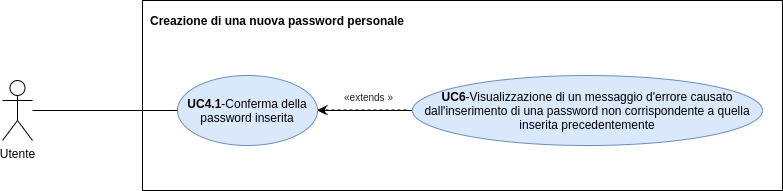
\includegraphics[width=\textwidth]{src/CasiDUso/immagini/SottocasoCreazionePassword.png}
	\caption{Zoom-in creazione password.}
\end{figure}


\subsubsection{UC-.1 Inserimento mail di registrazione}
\begin{itemize}
	\item \textbf{Attore primario:} utente non autenticato;

	\item \textbf{Descrizione:} l'utente vuole inserire il proprio indirizzo email su cui farsi mandare il link di recupero password;

	\item \textbf{Precondizioni:} l'utente ha cliccato sul link per la reimpostazione della password;

	\item \textbf{Postcondizioni:} l'utente ha inserito con successo la propria mail di registrazione;

	\item \textbf{Scenario principale:}
	      \begin{enumerate}
		      \item l'utente seleziona il campo dati in cui inserire la propria mail di registrazione;
		      \item l'utente inserisce la propria mail di registrazione;
		      \item l'utente invia i dati al sistema;
		      \item il sistema controlla la presenza dell'indirizzo email all'interno del database e, qualora fosse presente, invierà il link di recupero password;
	      \end{enumerate}
	\item \textbf{Estensioni:}
	      \begin{enumerate}
		      \item UC- Errore: inserimento di una mail non censita all'interno del sistema.
	      \end{enumerate}
\end{itemize}

\subsubsection{UC-.2 Inserimento di una nuova password}
\begin{itemize}
	\item \textbf{Attore primario:} utente non autenticato;

	\item \textbf{Descrizione:} l'utente vuole inserire una nuova password nell'apposito box;

	\item \textbf{Precondizioni:} l'utente ha cliccato sul link ricevuto tramite email per la reimpostazione della password;

	\item \textbf{Postcondizioni:} l'utente inserito con successo la nuova password;

	\item \textbf{Scenario principale:}
	      \begin{enumerate}
		      \item l'utente seleziona il campo dati in cui inserire la nuova password;
		      \item l'utente inserisce la nuova password;
		      \item il sistema controlla la password inserita e restituisce un messaggio di errore esplicativo nel caso non rispetti dei vincoli;
	      \end{enumerate}
	\item \textbf{Estensioni:}
	      \begin{enumerate}
		      \item UC- Errore: inserimento di una nuova password non valida.
	      \end{enumerate}
\end{itemize}

\subsubsection{UC- Errore: inserimento di una mail non censita all'interno del sistema}
\begin{itemize}
	\item \textbf{Attore primario:} utente non autenticato;

	\item \textbf{Descrizione:} l'utente ha inserito una mail non censita all'interno del sistema o contenente dei caratteri speciali non accettati dal sistema;
%TODO password valida se mettiamo password troppo lunga/corta/caratteri non validi
	\item \textbf{Precondizioni:} l'utente ha inserito una mail non presente nel sistema per il recupero della password;

	\item \textbf{Postcondizioni:} il sistema non accetta l'indirizzo email fornito dall'utente restituendo un errore esplicativo a video;

	\item \textbf{Scenario principale:}
	      \begin{enumerate}
		      \item l'utente seleziona il campo dati dove inserire la propria mail;
		      \item l'utente inserisce una mail non presente all'interno del sistema;
		      \item il sistema visualizza un messaggio di errore esplicativo e non invia il link di recupero.
		\end{enumerate}
		
\end{itemize}

%TODO da valutare se sdoppiarlo nel caso in cui l'utente non sia autenticato e voglia recuperare la password e nel caso in cui voglia modificare la password da autenticato.
\subsubsection{UC-.3 Conferma della modifica della password personale}
\begin{itemize}
	\item \textbf{Attore primario:} utente non autenticato;

	\item \textbf{Descrizione:} l'utente vuole confermare la password inserita riscrivendola sull'apposito box;

	\item \textbf{Precondizioni:} l'utente ha inserito una nuova password valida all'interno della pagina per l'inserimento di una nuova password;

	\item \textbf{Postcondizioni:} il sistema ha modificato con successo la password;

	\item \textbf{Scenario principale:}
	      \begin{enumerate}
		      \item l'utente re-inserisce la password precedentemente inserita nell'apposito box di conferma;
		      \item l'utente invia i dati al sistema;
		      \item il sistema analizza il matching tra le due password e in caso di errore restituisce un messaggio esplicativo e richiede nuovamente l'inserimento di una nuova password senza precedentemente completare la modifica della password. Se le password sono valide e coincidono, il sistema le conferma.
	      \end{enumerate}
	\item \textbf{Estensioni:}
	      \begin{enumerate}
	      %TODO UC5-5 posizionato in maniera corretta?
	      \item UC- Errore: inserimento di una password non corrispondente a quella inserita precedentemente.
	      \end{enumerate}
\end{itemize}

%TODO attore sistema? sdoppiare anche questo UC come discusso sopra?
\subsection{UC- Errore: inserimento di una password non valida nel sistema}
\begin{itemize}
	\item \textbf{Attore primario:} utente non autenticato;

	\item \textbf{Descrizione:} il sistema verifica se la password inserita rispetta i vincoli di lunghezza o complessità. Se la password non rispetta tali vincoli il sistema restituisce un errore;

	\item \textbf{Precondizioni:} l'utente ha inserito una password non valida durante l'impostazione di una nuova password.

	\item \textbf{Postcondizioni:} il sistema restituisce un messaggio d'errore esplicativo e chiede all'utente di inserire una nuova password valida senza apportare le modifiche;

	\item \textbf{Scenario principale:}
	      \begin{enumerate}
		      \item il sistema elabora la richiesta ricevuta;
		      \item il sistema restituisce un messaggio d'errore esplicativo che viene visualizzato sullo schermo del dispositivo dell'utente e non completa la registrazione del nuovo utente fino a quando non viene inserita una password corretta.
	      \end{enumerate}
\end{itemize}

%TODO idem a sopra
\subsection{UC- Errore: inserimento di una password non corrispondente a quella inserita precedentemente}
\begin{itemize}
	\item \textbf{Attore primario:} utente;

	\item\textbf{Descrizione:} l'utente vuole confermare la password inserita. Viene visualizzato un messaggio d'errore causato dall'inserimento di una password di conferma errata;

	\item\textbf{Precondizioni:} l'utente ha inserito una nuova password valida all'interno della pagina per l'inserimento di una nuova password e ha inserito una password di conferma diversa da quella inserita precedentemente;

	\item\textbf{Postcondizioni:} viene visualizzato un messaggio d'errore causato dall'inserimento di una password di conferma errata;

	\item \textbf{Scenario principale:}
	      \begin{enumerate}
		      \item l'utente inserisce la password precedentemente inserita;
		      \item il sistema analizza il matching tra le due password, in caso negativo restituisce un messaggio d'errore esplicativo e richiede nuovamente l'inserimento di una nuova password senza precedentemente completare la modifica della password.
	      \end{enumerate}
\end{itemize}

\subsection{UC- Logout mobile}
\begin{itemize}
	\item \textbf{Attore primario:} utente autenticato;

	\item \textbf{Descrizione:} l'utente vuole effettuare il logout da applicazione mobile;

	\item \textbf{Precondizioni:} l'utente è autenticato presso il sistema;

	\item \textbf{Postcondizioni:} l'utente non è più autenticato presso il sistema;

	\item \textbf{Scenario principale:}

	      \begin{enumerate}
		      \item l'utente seleziona la funzionalità di logout;
		      \item il sistema elabora la richiesta e aggiorna la schermata riportandola a quella d'avvio dell'applicazione e rendendo indisponibile l'accesso alla dashboard dell'utente fino a nuovo accesso.
	      \end{enumerate}
\end{itemize}